\scanpage{118}


$\otimes$-\uline{catégories}.

1) Définition. Catégorie \deleted{additiv} additive, avec bifoncteur
\[
(X,Y)\handwritten{\mapsto}X\otimes Y
\]
\deleted{et} un \deleted{objet} isomorphisme de bifoncteurs
\[
\handwritten{\phi}(X,Y,Z): (X\otimes Y)\otimes Z\handwritten{\xrightarrow{\sim}}X\otimes(Y\otimes Z)
\]
et un isomorphisme de commutativité
\[
\handwritten{\psi}(X,Y): X\otimes Y\handwritten{\xrightarrow{\sim}}Y\otimes X
\]
satisfaisant des axiomes

a) Axiome du pentagone pour $\handwritten{\phi}$ \deleted{(ne dépend pas de la structure additive),}

b) $\handwritten{\psi}(X,Y)\handwritten{\psi}(Y,X)=\mathrm{id}_{\unsure{\deleted{X}Y|\deleted{Y}X|X}\otimes X}$ \handwritten{;}

c) compatibilité entre $\handwritten{\phi}$ et $\handwritten{\psi}$ \handwritten{; axiome de l'hexagone}

d) existence d'un élément $1_C=\underline{1}$ , avec des isomorphismes fonctoriels
\[
u(X):\deleted{\unsure{x|=|-}}\quad\underline{1}\otimes X\handwritten{\simeq}X
\qquad\text{d'où}\quad
\inserted{v(X)=}\handwritten{\psi}(X,1)u(X): X\otimes1\handwritten{\simeq}X\ ,
\]
\figure{\handwritten{
\begin{tikzpicture}[x=1cm,y=1cm]
\draw (-.75,.05) .. controls (-.9,.7) and (.3,.3) .. (.5,.6);
\draw (-.6,.05) .. controls (-.4,-.45) and (.75,-.4) .. (.85,0) .. controls (.95,.6) and (1.5,.7) .. (1.85,.3);
\draw[line width=.15pt] (1.12,.57)--(1.48,.28);
\draw[line width=.15pt] (.03,-.49) .. controls (.29,-.63) and (.56,-.52) .. (.69,-.43);
\end{tikzpicture}}}
(donc par b on aura aussi $u(X)=v(X)\handwritten{\psi}(1,X)$)

avec la condition que pour $X=\underline{1}$, on trouve le même isomorphisme
\[
\makebox[0pt][r]{\begin{tikzpicture}[x=1em,y=1em]\fill (0,0) circle (.045);\end{tikzpicture}\hspace{3em}}
u(\underline{1})=v(\underline{1}) :\qquad \underline{1}\otimes\underline{1}\handwritten{\simeq}\underline{1}
\]
ce qui s'exprime aussi par la condition que $\handwritten{\psi}(\underline{1},\underline{1})=\mathrm{id}_{\underline{1}}$ \handwritten{;}

\margin{\handwritten{de plus on veut\figure{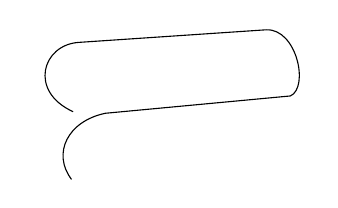
\begin{tikzpicture}[x=1cm,y=1cm]
\draw (-1.23,-.23) .. controls (-1.8,.03) and (-1.62,.62) .. (-1.16,.65) -- (1.22,.81) .. controls (1.61,.83) and (1.77,.08) .. (1.53,-.03) -- (-.82,-.25) .. controls (-1.3,-.35) and (-1.5,-.76) .. (-1.25,-1.09);
\end{tikzpicture}}}}
\inserted{\handwritten{Compatibilité de $(\underline{1},u,v)$ avec $\phi$, quand $X,Y$ \unsure{ou|,-} $Z$ \unsure{est} \unsure{égal|ég.} à $1$, avec $\psi$ pour $X$ \unsure{ou|,-} $Y$ est $=1$.}}

e) le foncteur $\otimes$ est biadditif.

\margin{\handwritten{Envisager aussi \unsure{les structures éventuelles|la structure éventuelle} $\underline{\mathrm{Hom}}(X,Y)$, relation avec $\check{X}\otimes Y$\figure{\begin{tikzpicture}[x=1cm,y=1cm]
\draw (-1.6,1.45) -- (.8,1.8) -- (1,1.05) -- (1.9,1.15) .. controls (.95,.6) and (1.2,.3) .. (1.1,-.5) -- (-1.5,-1.8);
\end{tikzpicture}}}}

NB a) \deleted{et d) sont}\inserted{est} indépendant\deleted{s} de la donnée de $\handwritten{\psi}$ , b) est indépendant de la donné de $\handwritten{\phi}$ , a)b)c)d) sont indépendant d\unsure{\deleted{e}u|\deleted{u}e} \unsure{\deleted{l}f|f}\unsure{\deleted{'}a|a}it que $C$ est additiv\deleted{\unsure{t|i}}e.

Soit $\underline{1}',u',\inserted{v'\handwritten{\begin{tikzpicture}[x=.4cm,y=.4cm,baseline=-.2ex]\draw (0,-.2) .. controls (-.28,.4) and (.1,.65) .. (.53,1.01);\end{tikzpicture}}}$ comme $\underline{1},u,v$ , on va \deleted{définir canoniquement un}\inserted{\handwritten{\unsure{voir|voit} qu'il existe un unique}} isomorphisme $w:\underline{1}\handwritten{\simeq}\underline{1}'$ , compati\unsure{\deleted{v}b|b}le en un sens évident avec $u,v$ et $u',v'$.

On choisit le composé
\diagram{\begin{tikzcd}[ampersand replacement=\&]
\underline{1} \arrow[r,"{\handwritten{v'(\underline{1})}}"] \&
\underline{1}\otimes\underline{1}' \arrow[r,"{\handwritten{\unsure{\deleted{\underline{1}\otimes u'}u(\underline{1}')|u(\underline{1}')|v(\underline{1}')}}}"] \&
\underline{1}'\deleted{\otimes\unsure{\underline{1}}} \arrow[r,phantom,"{\deleted{\longrightarrow}}" description,"{\deleted{\handwritten{\unsure{u}}}}"] \& \deleted{\unsure{\underline{1}'}}
\end{tikzcd}}
. A vérifier les compatibilités annoncées (ne dépend pas de la donnée de $\handwritten{\phi}$, \inserted{ni $\handwritten{\psi}$,\handwritten{\begin{tikzpicture}[x=.4cm,y=.4cm,baseline=-.2ex]\draw (0,-.2) .. controls (-.18,.36) and (.2,.46) .. (.42,.48) .. controls (.93,.5) and (1.34,.62) .. (1.27,.79);\end{tikzpicture}}} mais de $u,v$ satisfaisant la compatibilité $\underline{u}(\underline{1})=v(\underline{1})$\deleted{\unsure{\mbox{
\begin{tikzpicture}[x=.5em,y=.5em,baseline=-.2ex]
\draw (.17,.57) ellipse (.16 and .21);
\draw (.08,-.25) .. controls (.28,.05) and (.17,.76) .. (.13,1.02);
\draw (.13,1.02) .. controls (.18,.91) and (.3,.91) .. (.38,1.04);
\draw (.23,.73)--(.43,.79);
\draw (.81,.61)--(.48,.24)--(.79,.24) .. controls (1,.08) and (.76,-.08) .. (.68,-.05);
\end{tikzpicture}}|,}} et $u',v'$ kif-kif). C'est pourquoi il n'y\inserted{a\handwritten{\begin{tikzpicture}[x=.4cm,y=.4cm,baseline=-.2ex]\draw (0,-.2) .. controls (.05,.21) and (.31,.65) .. (.53,.94);\end{tikzpicture}}} pas lieu de poser $\underline{1},u,v$ comme donnée, mais comme axiome d'existence.
